We are concerned with learning generative models that describe transformations of a source-language sequence $\ve=(e_1,\ldots, e_I)$ to a target-language sequence $\vf=(f_1,\ldots,f_J)$. We consider two different data scenarios.

In the parallel data setting, each sample in the observed data consists of a pair $(\ve, \vf)$.
The generative story assigns the following probability to the event that $\vf$ arises from~$\ve$:
\begin{equation}
p(\vf \mid \ve; \Theta) = \sum_\va p(\va,\,\vf \mid \ve)
\label{eqn:parallel}
\end{equation}
where $\Theta$ denotes the model parameters and $\va$ denotes a hidden variable that corresponds to unknown choices taken in the generative process.
%(in our case, $\va$ is an alignment, see next subsection).

In the non-parallel data setting, only the target sequence $\vf$ is observed and the source sequence $\ve$ is hidden. 
The model assigns the following probability to the observed data:
\begin{equation}
p(\vf; \Theta) = \sum_{\ve} p(\ve) \sum_{\va} p(\va,\,\vf \mid \ve).
\label{eqn:decipherment}
\end{equation}
That is, the sequence $\vf$ can arise from any sequence $\ve$ by first selecting $\ve \sim p(\ve)$ and then proceeding according to the parallel-data generative story (\eqn{eqn:parallel}).

Unsupervised training of such models entails maximizing the data log-likelihood $L(\Theta)$:
\begin{align*}
\arg\max_{\Theta}\,\,L(\Theta)
%=&\max_{\Theta}\,\,\log\prod_{n}p (\vx_n;\Theta)\\
=&\arg\max_{\Theta}\,\,\sum_{x\in X}\log p (\vx;\Theta)
\end{align*}
%_{n=1}^{N}
where $X=\set{(\ve^n,\vf^n)}_n$ in the parallel data setting and $X=\set{(\vf^n)}_n$ in the non-parallel data setting.

Although the structure of $\Theta$ is unspecified, in practice, most models that follow these generative stories contain a source-to-target translation table (``t-table'') denoted $t$, with each parameter $t(f\mid e)$ representing the conditional probability of mapping a given source symbol $e$ to target symbol~$f$. 
%Henceforth, we assume each model $\Theta$ contain such a t-table parameter



%We make the discussion concrete by discussing two related tasks - word alignment and back-transliteration. 

%The predominant approach for training these generative models 


%%%%%%%%%% BACKUP from ACL
%\subsection{Generative Models}
%%\marginpar{DC: In my opinion, this subsection could be dropped}
%
%We are concerned with learning generative models that describe transformations of a source-language sequence $\ve$ to a target-language sequence $\vf$.
%We consider two different settings for these models.
%
%In the parallel data setting, both $\ve$ and $\vf$ are observed, so that the data consists of instances $\vx = (\ve, \vf)$. 
%The generative story assigns the following probability to the event that $\vf$ arises from~$\ve$:\footnote{With a slight notation abuse for $p(\vx;\Theta).$}
%%\marginpar{DC: one way to fix the abuse of notation is to explicitly write $p(\ve)$ here.}
%\begin{equation}
%p(\vx; \Theta) = p(\vf \mid \ve) = \sum_\va p(\va,\,\vf \mid \ve)
%\label{eqn:parallel}
%\end{equation}
%where $\Theta$ denotes the model parameters and $\va$ denotes a hidden variable that corresponds to unknown choices taken of the generative process.
%%(in our case, $\va$ is an alignment, see next subsection).
%
%In the non-parallel data setting, only the target entity $\vf$ is observed and the source entity $\ve$ is considered hidden. 
%Letting $\vx = (\vf)$, the model takes the form:
%\begin{equation}
%p(\vx; \Theta) = p(\vf) = \sum_{\ve} p(\ve) \sum_{\va} p(\va,\,\vf \mid \ve)
%\label{eqn:decipherment}
%\end{equation}
%That is, the observed entity $\vf$ can arise from any source entity $\ve$ by first selecting $\ve \sim p(\ve)$ and then proceeding according to the parallel data generative story.
%
%Training these models entails the same objective function -- maximizing the observed data log-likelihood $L(\Theta \mid X)$:
%\begin{align*}
%\max_{\Theta}\,\,L(\Theta \mid X)
%%=&\max_{\Theta}\,\,\log\prod_{n}p (\vx_n;\Theta)\\
%=&\max_{\Theta}\,\,\sum_{n}\log p (\vx^n;\Theta)
%\end{align*}
%%_{n=1}^{N}
%where $X=\set{(\ve^n,\, \vf^n)}_n$ in the parallel data setting and $X=\set{(\vf^n)}_n$ in the non-parallel data setting.
%
%Next, we make these generative stories concrete by explicitly defining $p(\va, \vf \mid \ve)$ and $p(\ve)$ (if necessary) in two sequence alignment tasks -- word alignment and back-transliteration decipherment.
%
%%We make the discussion concrete by discussing two related tasks - word alignment and back-transliteration. 
%
%%The predominant approach for training these generative models 
%
%\subsection{Parallel Data: Word Alignment}
%
%%Keeping the discussion abstract, we consider the general problem of sequence alignment. 
%%In sequence alignment, we are given a sequence $e = (e_1, \ldots, e_I)$ comprising of source language entities and a sequence $f = (f_1, \ldots, f_J)$ comprising of target language entities (concretely, these entities can represent words or phonemes in each language) and are tasked with finding an alignment 
%
%Word alignment is one of the major building blocks in the conventional machine translation pipeline.
%In word alignment, the sequence $\ve = (e_1, \ldots, e_I)$ is a sentence in the source language and $\vf = (f_1, \ldots, f_J)$ is a sentence in the target language. 
%The generative story for the transformation of $\ve$ to $\vf$ follows \eqn{eqn:parallel}, where the hidden variable $\va = (a_1, \ldots, a_J)$ is a sequence of $J$ indices which indicates that the $j$th target word is aligned to the $a_j$th source word. 
%In other words, under the generative story, $f_j$ is thought to be generated from $e_{a_j}$.
%
%%The HMM word alignment model is considered both computationally efficient and effective. However, since its objective is not convex, it is common practice to initialize training using the simpler IBM 1 model.
%The IBM word alignment models \cite{brown+alii:1993} and the HMM word alignment model \cite{vogel+alii:1996} assign the following conditional probability for a target sequence $\vf$ given an observed source sequence $\ve$ and a fixed alignment $\va$:
%\begin{equation}
%p(\va, \vf \mid \ve) = \prod_{j=1}^{J} t(f_j \mid e_{a_j})\cdot a(a_j \mid a_{j'})
%\label{eqn:WA}
%\end{equation}
%That is, they are parameterized using two conditional probability distributions $\Theta=(t, a)$. 
%The translation table $t(f_j \mid e_{a_j})$ encodes the probability of translating $e_{a_j}$ to $f_j$, and $a$ is a model-dependent probability distribution that quantifies the probability of aligning the $j$th target position with the $a_j$th source position, possibly given a previous alignment decision. In this paper, we are only concerned with $t$.
%
%\iffalse
%IBM Model 1 uses a degenerate distortion table that assigns a uniform probability to all possible source positions, and the HMM model encodes distortions using a first-order dependency on the previously non null-aligned position $a_{j'}$.
%The exact details behind the HMM distortion parameters are implementation specific and therefore beyond the scope of this paper. See \cite{och+ney:2003,liang+:2006:align} for the respective GIZA++ and ABA implementation details.
%\fi
%
%\subsection{Non-Parallel Data: Back-Transliteration}
%
%\begin{figure*}
%\begin{center}
%\begin{tabular}{c}
%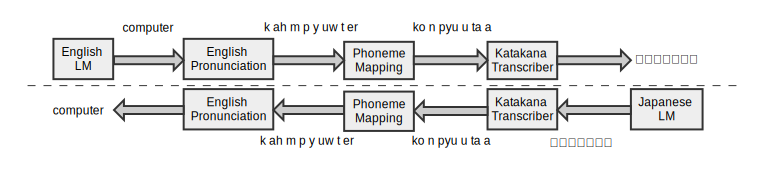
\includegraphics[scale=0.62]{figures/fsts}\tabularnewline
%\end{tabular}
%\caption{\label{font-table} The transliteration generative story as a cascade of wFSTs. Each box represents a transducer. \textbf{Top:} transliteration of the word ``computer'' to Japanese. \textbf{Bottom:} the reverse process. PAT jointly trains the two cascades by maximizing both the data log-likelihood and the parameter agreement of the two (shaded) phoneme mapping models. The blank wFSTs are held fixed. }
%\label{fig:fsts}
%\end{center}
%\end{figure*}
%
%Transliteration is a mapping of terms between writing systems of different languages. 
%Usually, the mapping tries to preserve the sound of a term as it is uttered in the original language. 
%For example, the word ``computer'' in English is transliterated to Japanese as ``konpyuutaa'' (in Romaji). 
%The process restoring transliterated foreign words to their original script is called \emph{back-transliteration}.
%
%Knight and Graehl \shortcite{KG98} suggest a generative story for the transliteration of an English term $\vw$ into Japanese term $\vk$ (see top of Figure \ref{fig:fsts}): 
%\begin{enumerate}
%\item First, a word $\vw$ is generated according to an English language model (LM)
%$p(\vw)$.
%\item $\vw$ is then mapped to an English phonemes sequence $\ve=(e_1,\ldots,e_I)$ according to a pronunciation model.
%\item The phoneme sequence $\ve$ is mapped to a sequence of Japanese phonemes $\vj=(j_1,\ldots,j_J)$ according to a phoneme mapping model $p(j \mid e)$.
%\item Finally, the Japanese phoneme sequence $\vj$ is mapped to a
%Japanese word $\vk$ in Katakana.
%\end{enumerate}
%Each of their models is encoded as a weighted Finite-State Transducer (wFST) that can be constructed and trained independently. Knight and Graehl estimate wFSTs 1,2,4 over monolingual data only, whereas the phoneme mapping model $p(j \mid e)$ (\eqn{eqn:parallel}) is trained over a parallel phoneme corpus $\set{(\ve_{n},\, \vj_{n})}$ and further restricted such that each English phoneme is allowed to map to either one or two Japanese phonemes only.
%
%However, collecting parallel data is a time consuming, laborious process.
%To combat the need for parallel data, Ravi and Knight \shortcite{RK09} suggest to estimate model 2 from non-parallel data. %, for which only Japanese words $K=\set{\vk^n}_{n=1}^{|K|}$ need be collected. 
%Assuming one-to-one transformations for models 2 and 4 
%(so that $p(\vw) = p(\ve)$ and $p(\vk) = p(\vj)$) 
%the generative process for transliteration is identical to that of \eqn{eqn:decipherment}:
%\begin{align*}
%p(\vk)=p(\vj)
%=&\sum_\vw p(\vw) \cdot p(\vj \mid \vw)\\
%=&\sum_\ve p(\ve) \cdot p(\vj \mid \ve)\\
%=&\sum_\ve p(\ve) \sum_\va  p(\va,  \vj \mid \ve),
%\end{align*}
%\newcommand{\slice}[3]{\ensuremath{#1[#2\mathop{:}#3]}}
%Letting $\slice \vj{a}{b} =  j_a \cdots j_{b-1}$.
%The alignment $\va=(a_0, \ldots, a_I)$, where $a_{i} - a_{i-1} \in \{1, 2\}$ for $1 \leq i \leq I$,
%%where $\va=((\va_{1}^{\tstart}, \va_{1}^{\tend}),\ldots,(\va_{I}^{\tstart}, \va_{I}^{\tend}))$ 
%%denotes a \emph{source-to-target} monotone alignment sequence under which
%indicates that 
%$e_i$ is mapped to 
%%one or two phonemes from $\vj$, denoted $\vj[\va_{i}^{\tstart}:\va_{i}^{\tend}]$.
%the phonemes $\slice\vj{a_{i-1}}{a_i}$.
%% $\va_{i}^{\cdot} \le \va_{i+1}^{\cdot}$ and $1 \le \va_{i}^{\tstart} \le \va_{i}^{\tend} \le J$ for all $i$.
%The overall probability of this mapping is then:
%\begin{equation}
%%p(\va,  \vj \mid \ve) = \prod_{i=1}^{I} t(\vj[a_{i}^{\tstart}:a_{i}^{\tend}] \mid e_{i})
%p(\va,  \vj \mid \ve) = \prod_{i=1}^{I} t(\slice \vj{a_{i-1}}{a_i} \mid e_{i})
%\label{eqn:trans}
%\end{equation}
%where 
%%$t(\vj[a_{i}^\tstart:a_{i}^\tend] \mid \ve_{i})$ 
%$t(\slice\vj{a_{i-1}}{a_i} \mid \ve_{i})$ 
%is the probability of transliterating English phoneme $e_i$ to Japanese phoneme(s) 
%%$\vj[a_{i}^\tstart:a_{i}^\tend]$.
%$\slice\vj{a_{i-1}}{a_i}$.
%
%
%%Thus, a Japanese phoneme sequence $\vj$ can arise from any English pronunciation sequence $\ve$ that is producible by the language and pronunciation models:
%%$$
%%p(\vj) = \sum_{\ve} p(\ve)\cdot p(\vj \mid \ve)$$
%%As a result, the data log-likelihood takes the form:
%%\begin{align}
%%L(J)& = \sum_{\mathbf{j}\in J} \log \sum_{\mathbf{e}} \PP(\mathbf{j}\mid \mathbf{e})\cdot \PP(\mathbf{e})
%%\end{align}
%%Once the model is trained, back-transliteration (decoding) of Japanese words back to English can be done using the Viterbi algorithm.
%
%%We note a few points:
%%\begin{itemize}
%%\item The computational cost of solving this problem is much higher than the parallel case since we are forced to use the language and pronunciation models during training time. 
%%\item Only the phoneme mapping parameters $P(j_{m}\mid e_{m})$ are trained while
%%the other FSTs' parameters are kept fixed.
%%\end{itemize}
%
%
%
%
%
%
%
%
%
%%We briefly discuss two machine translation related tasks - word alignment and phonetic back-transliteration.
%%Both tasks share a similar generative story that describes how source sequences $e=(e_1, \ldots, e_I)$ (of strings or phonemes) are distorted (reordered) and translated into target sequences $f = (f_1, \ldots, e_J)$.
%%As shall be seen, their sole difference lies in the permitted set of distortions - whereas all alignments are permitted in word alignment, only monotone alignments are allowed in back-transliteration.
%
%
%
%%In machine learning, and machine translation in particular, generative stories describes transformations of entities $e$ (strings, phonemes) from a source language to entities $f$ in a target language.
%%The generative story explicitly construct conditional probability distributions $P(f\mid e)$ where $e$ is an entity from $L_{E}$ and $f$ is an entity from $L_{F}$.
%%The predominant approach for training generative models is the EM
%%framework which iteratively maximizes log-likelihood of the observed
%%data $X=\{e_{n},\, f_{n}\}_{n=1}^{N}$:
%%\begin{align*}
%%\max_{P}L(P\mid X)=\max_{P}\sum_{n}\log P(f_{n}\mid e_{n})
%%\end{align*}
%%In a setting like word alignment where models are trained in both directions, we adopt the notation $\PP(e_{n}\mid f_{n})$ for one direction and $\QQ(f_{n}\mid e_{n})$
%%for the other. 
%%The two models can be independently trained by maximizing each data log-likelihood function separately:
%%\begin{align*}
%%\PP^{*} &= \argmax_{\PP}L(\PP\mid X)\\
%%\QQ^{*} &= \argmax_{\QQ}L(\QQ\mid X).
%%\end{align*}
